\documentclass{article}
\usepackage[catalan]{babel}
\usepackage[latin1]{inputenc}   % Permet usar tots els accents i car\`acters llatins de forma directa.
\usepackage{enumerate}
\usepackage{amsfonts, amscd, amsmath, amssymb}
\usepackage{fancyheadings}
\usepackage{graphicx}

\setlength{\textwidth}{16cm}
\setlength{\textheight}{25cm}
\setlength{\oddsidemargin}{-0.3cm}
\setlength{\evensidemargin}{0.25cm} \addtolength{\headheight}{\baselineskip}
\addtolength{\topmargin}{-3cm}

\newcommand\Z{\mathbb{Z}}
\newcommand\R{\mathbb{R}}
\newcommand\N{\mathbb{N}}
\newcommand\Q{\mathbb{Q}}
\newcommand\K{\Bbbk}
\newcommand\C{\mathbb{C}}

\newcounter{exctr}
\setcounter{exctr}{11}
\newenvironment{exemple}
{ \stepcounter{exctr} 
\hspace{0.2cm} 
\textit{Exemple  \arabic{exctr}: }
\it
\begin{quotation}
}{\end{quotation}}

\pagestyle{fancy}
\markboth{Tema 4. An\`alisi i processament de senyals aleatoris}{}
\setcounter{page}{1}
\setlength{\headrulewidth}{0pt}



\begin{document}


\textbf{\Large Tema 4. An\`alisi i processament de senyals aleatoris}

\vskip 0.5 cm

\textbf{\large La import\`ancia dels processos estoc\`astics en l'estudi dels sistemes de comunicacions}

Un sistema de comunicacions es composa d'un senyal d'informaci\'o que s'envia a trav\'es d'un canal de
transmissi\'o des d'un emissor fins a un receptor. Esquem\`aticament:
\begin{figure}[htbp]
\centerline{
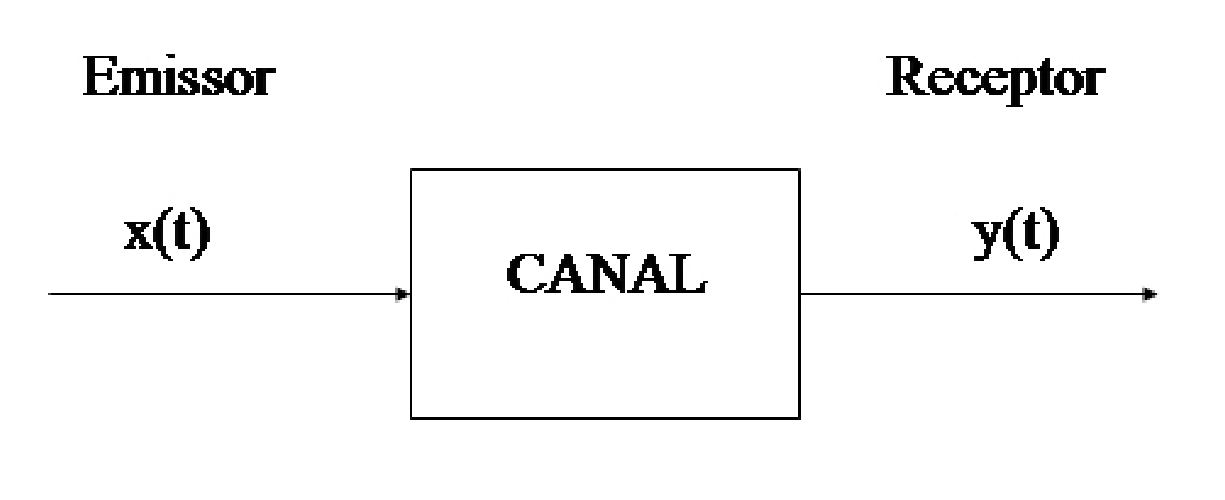
\includegraphics[width=6cm]{esqcomunic.eps}
}
\end{figure}

L'efecte del canal damunt el senyal original es modela mitjan\c{c}ant una funci\'o $h(t)$. Si el canal \'es
un sistema lineal invariant en el temps (LTI), llavors $h(t)$ rep el nom de {\bf resposta impulsional} del canal.
La relaci\'o entre $x(t)$ i $y(t)$ \'es:
\[
y(t)=h(t) \ast x(t) = \int_{-\infty}^{+\infty} x(s) h(t-s) ds
\]

Una altra manera d'expressar la relaci\'o entre l'entrada i la sortida del canal \'es utilitzant la transformada 
de Fourier. Per propietats d'aquesta transformada es t\'e:
\[
Y(f)=H(f) \cdot X(f)
\]
\noindent
on $X(f)$, $Y(f)$ i $H(f)$ s\'on les transformades respectives de $x(t)$, $y(t)$ i $h(t)$.

\vskip 0.2 cm
Qualsevol canal de transmissi\'o real, a part de modificar el senyal original segons una certa funci\'o $h(t)$,
tamb\'e modifica de manera aleat\`oria aquest senyal. Es diu llavors que el canal introdueix {\bf renou}.
Una manera freq\"uent de modelar un canal real \'es la seg\"uent:

\begin{figure}[htbp]
\centerline{
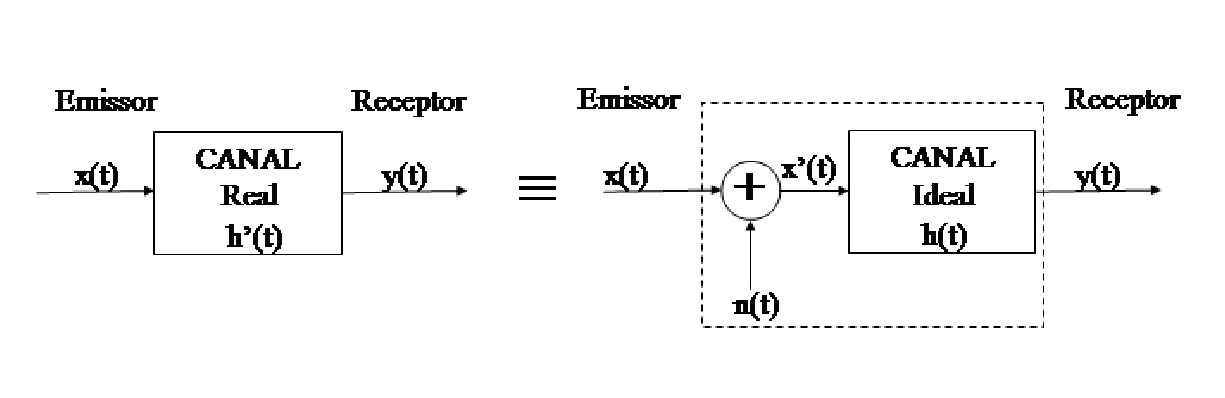
\includegraphics[width=9cm]{esqrenou.eps}
}
\end{figure}

\'Es a dir, l'efecte del canal es modela afegint un terme aleatori $n(t)$ al senyal original. La suma d'aquests
dos termes \'es el que entra en un canal ideal (no soroll\'os) amb resposta impulsional $h(t)$.
Per tant:
$$y(t)=h(t) \ast x'(t)$$ on
$$x'(t)=x(t) + n(t)$$

La funci\'o $n(t)$ \'es una funci\'o que varia de manera aleat\`oria al llarg del temps. Es tracta per tant
de la realitzaci\'o d'un {\bf proc\'es aleatori}. {\bf L'estudi dels processos aleatoris ens permet} per tant 
{\bf estudiar el comportament del renou en sistemes de comunicacions}.
En molts de casos $n(t)$ es modela com un proc\'es gaussi\`a, per les seves propietats d'ergodicitat, que fan senzill
l'estudi del seu comportament.

\vskip 0.2 cm
El comportament del renou quan passa pel canal ve determinat per l'expressi\'o:
\[
y(t)=h(t) \ast (x(t) + n(t)) = h(t) \ast x(t) + h(t) \ast n(t) = y_{\mathrm{id}}(t) + n_{\mathrm{canal}}(t)
\]
\noindent
on $y_{\mathrm{id}}(t)$ \'es la sortida del canal ideal (sense renou) i $n_{\mathrm{canal}}(t)$ \'es el renou de
sortida del canal. Idealment es dessitja que aquest darrer terme sigui el m\'es petit possible, per aconseguir-ho
s'afegeixen a la sortida del canal uns sistemes anomenats {\bf filtres} que modifiquen $h(t)$ per aconseguir que el 
renou de sortida sigui petit.

Des del punt de vista freq\"uencial, l'expressi\'o $n_{\mathrm{canal}}(t)=h(t) \ast n(t)$ s'escriu:
\[
N_{\mathrm{canal}}(f)=H(f) \cdot N(f)
\]
\noindent
on $N(f)$ \'es la transformada de Fourier de $n(t)$.

El problema \'es que $n(t)$ no \'es m\'es que una realitzaci\'o d'un proc\'es aleatori i pot tenir diferents formes,
per tant no ens d\'ona una informaci\'o v\`alida relativa al proc\'es. Per aquest motiu, en lloc de calcular $N(f)$
es calcula la seg\"uent transformada:
\[
S_N(f)={\cal TF}\{R_N(\tau)\}
\]

$S_N(f)$ s'anomena {\bf densitat espectral de pot\`encia} del proc\'es aleatori i \'es igual a la transformada
de Fourier de la funci\'o d'autocorrelaci\'o.

La ra\'o d'utilitzar $S_N(f)$ en lloc de $N(f)$ \'es que la funci\'o d'autocorrelaci\'o reflecteix b\'e el comportament
temporal del proc\'es: si el proc\'es canvia r\`apidament llavors esdev\'e r\`apidament incorrelat amb si mateix
i $R_X(\tau)$ decreix r\`apidament; en canvi, si el proc\'es varia lentament amb el temps llavors es mant\'e correlat
amb s\'i mateix durant un per\'\i ode gran i $R_X(\tau)$ decreix lentament. Aix\'o \'es degut a la propietat seg\"uent:
\[
P(X(t) X(t+\tau) > \varepsilon) \leq \frac{\tau}{\varepsilon^2} (R_X(0)-R_X(\tau))
\]

Per tant, la transformada de Fourier de $R_X(\tau)$ (la densitat espectral de pot\`encia) reflexa les freq\"u\`encies
implicades en el canvi del proc\'es aleatori: altes freq\"u\`encies indiquen canvis r\`apids mentre que baixes
freq\"u\`encies indiquen canvis lents, igual que per a qualsevol altra senyal no aleat\`oria. En conclusi\'o:
\[
N_{\mathrm{canal}}(f)=H(f) \cdot S_N(f)
\]

\vskip 0.5 cm

\textbf{\large Renou blanc Gaussi\`a}

\vskip 0.2 cm
\'Es habitual que en molts de problemes de comunicacions el renou es modeli com un 
\textit{renou blanc Gaussi\`a amb mitjana $0$ i densitat espectral de pot\`encia $\frac{N_0}{2}$}.
Aix\'o significa que el renou es modela com un proc\'es aleatori Gaussi\`a $X(t)$, estacionari,  
amb una distribuci\'o de pot\`encia constant per a totes les freq\"u\`encies: $S_X(f)=\frac{N_0}{2}$.

\vskip 0.2 cm
En conseq\"u\`encia:

\[
R_X(\tau)={\cal TF}^{-1} \{ S_N(f) \} = \frac{N_0}{2} \delta(t)
\qquad \qquad \text{en particular:} \qquad R_X(0)=\frac{N_0}{2}
\]

\vskip 0.2 cm
D'altra banda:
\[
\begin{array}{ll}
R_X(0)&= R_X(t, t)=E(X(t) \cdot X(t))=E( (X(t))^2 ) = \mathrm{Var}(X(t)) + E(X(t))^2 = \\ \\
&=\text{(el proc\'es t\'e mitjana 0)}=\mathrm{Var}(X(t))
\end{array}
\]

\vskip 0.3 cm
En conclusi\'o:
\[
X(t) \sim N(0, \frac{N_0}{2} )
\]



\end{document}